\chapter{机器人核心参数}
\section{机械参数} 
% 官方要求：重量、重心；尺寸（长宽高）；主要传感器型号、参数、数量。
本赛季团队研发的哨兵是中心供弹式、全向轮底盘式的哨兵，其机械结构设计紧凑，合理且有效地利用空间。
\subsection{基本参数}


\begin{table}[hbtp!]
    \renewcommand\arraystretch{1.5}
    \centering
    \begin{tabular}{ m{2cm}  m{10cm} }
    \toprule
      基本参数    &   参数量化  \\
     \midrule
     尺寸       & 长：$\qty{549.243}{\mm}$，宽：$\qty{580.000}{\mm}$，高：$\qty{697.009}{\mm}$，如  \figref{fig:rm_ci_机器人核心参数}所示 \\ \\
     质量       &  $\qty{17.5}{\kg} $     \\  \\
     重心位置   &  位于Yaw轴所在轴线上，且离地$\qty{200.000}{\mm} $      \\ 
    \toprule
    \end{tabular}
    \caption{机械基本参数}
    \label{tab:基本参数_机器人核心参数}
\end{table}

\begin{figure}[hbt!]
    \centering
    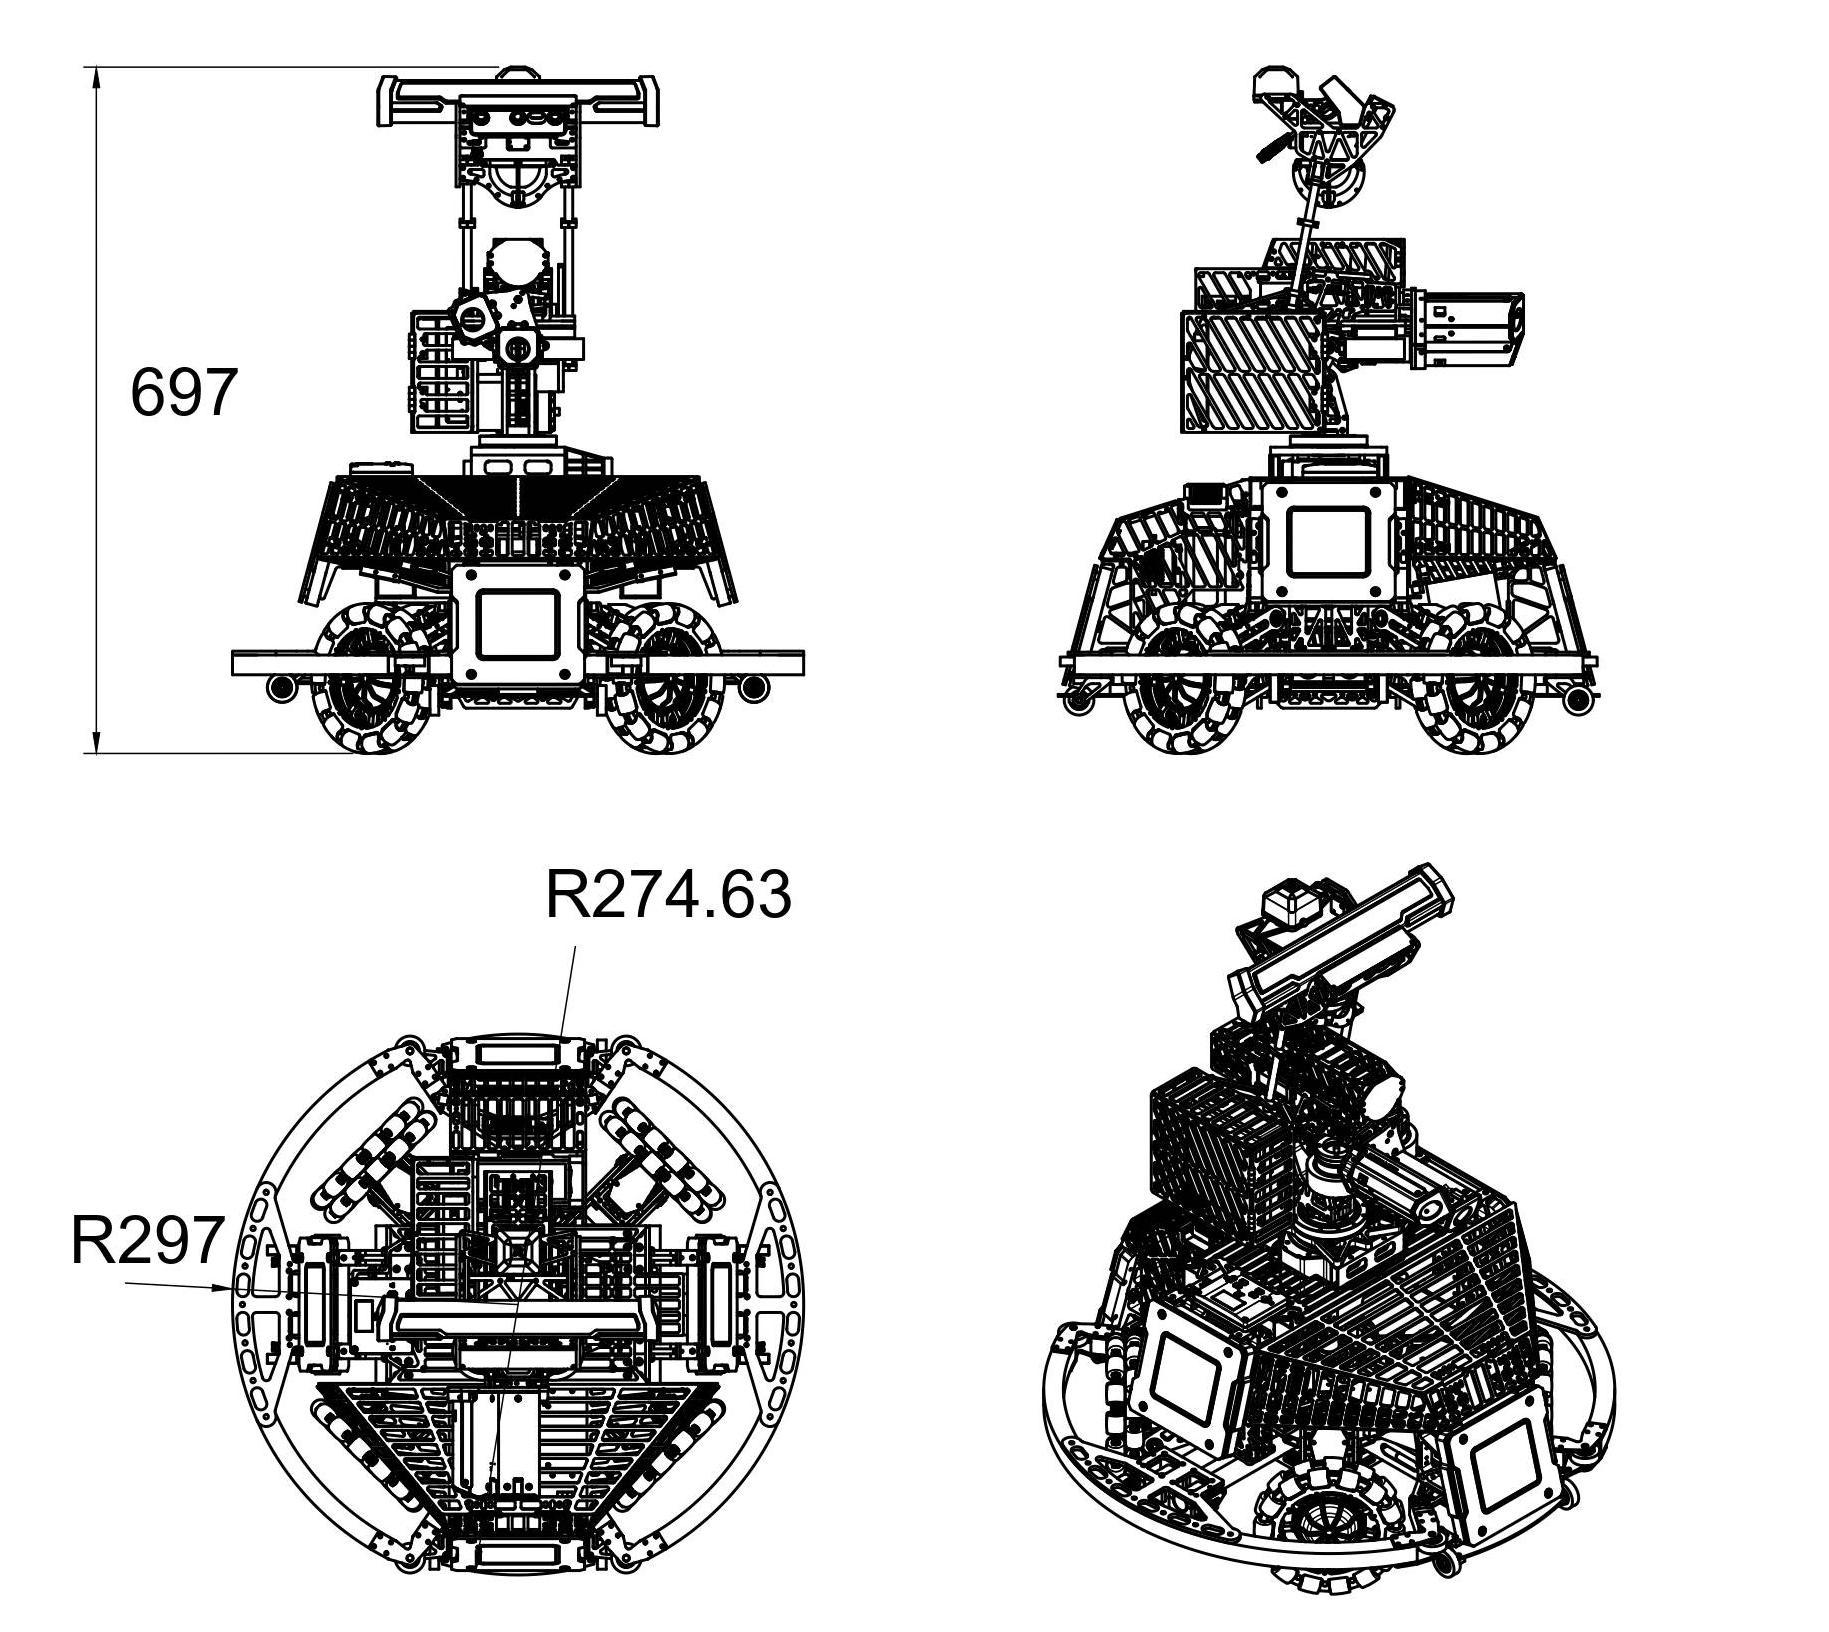
\includegraphics[width=0.9\columnwidth]{figure/机器人核心参数/机器人核心参数.jpg}
    \caption{机器人尺寸}
    \label{fig:rm_ci_机器人核心参数}
\end{figure}

% \newpage
\subsection{机械执行器件}

\begin{table}[hbtp!]
    \renewcommand\arraystretch{1.5}
    \centering
    \begin{tabular}{ m{3cm} m{4cm} m{2cm} }
    \toprule
    执行元件 &  用途  &  数量（个）  \\
    \midrule
    \multirow{2}*{M2006电机}
       &为拨盘提供动力源      & 1 \\ 
       &驱动双测速模块互相切换      & 1 \\ 
    \midrule
    \multirow{3}*{M3508电机}
       &为整车的全向移动提供动能      & 4 \\ 
       &驱使Pitch轴转动           & 1 \\ 
       &为弹丸提供初始动能        & 2 \\ 
    \midrule
    \multirow{1}*{GM6020电机}
       &驱使云台周转运动      & 1 \\ 
    \toprule
    \end{tabular}
    \caption{机械执行器件}
    \label{tab:机械执行器件_机器人核心参数}
\end{table}  